\documentclass[11pt,xcolor=dvipsnames]{beamer}

\usetheme{Copenhagen}

\usepackage[utf8]{inputenc}
\usepackage[italian]{babel}
\usepackage{listings,color}

\setbeamercovered{transparent}
%Maroon BrickRed OliveGreen MidnightOliveGreen
\usecolortheme[named=OliveGreen]{structure}
\usenavigationsymbolstemplate{}
\setbeamertemplate{headline}{}
\setbeamertemplate{footline}[frame number]
\setbeamertemplate{itemize items}[circle]
\setbeamertemplate{enumerate items}[circle]
\setbeamercolor{block body}{fg=white,bg=OliveGreen}
\pdfcompresslevel=0

\title{PAES}
\author{Paolo Bernardi}
\subtitle{Analisi e sviluppo di un'implementazione parallela dell'AES per architetture eterogenee 
multi/many-core}
\institute{Università degli Studi di Perugia --- Laurea Specialistica in Informatica}
\date{11 febbraio 2010}

\usepackage{avant}

\frenchspacing
\linespread{1.3}

\lstdefinelanguage{opencl}{
	morekeywords={__kernel, __constant, __global, __local, __private, __attribute__, vec_type_hint},
	sensitive=false
}

\lstset{
	numberstyle=\footnotesize,      % the size of the fonts that are used for the line-numbers
	numbersep=5pt,                  % how far the line-numbers are from the code
	backgroundcolor=\color{white},  % choose the background color. You must add \usepackage{color}
	showspaces=false,               % show spaces adding particular underscores
	showstringspaces=false,         % underline spaces within strings
	showtabs=false,                 % show tabs within strings adding particular underscores
	tabsize=4,                      % sets default tabsize to 2 spaces
	captionpos=b,                   % sets the caption-position to bottom
	breaklines=true,                % sets automatic line breaking
	breakatwhitespace=false,        % sets if automatic breaks should only happen at whitespace
	escapeinside={\%*}{*)},         % if you want to add a comment within your code
	basicstyle=\fontfamily{phv}\selectfont,
	language=C,
	alsolanguage=opencl
}

\begin{document}

\setbeamercolor{normal text}{bg=white}
\begin{frame}[plain]
\end{frame}
\setbeamercolor{normal text}{bg=white}

\begin{frame}[plain]
	%\titlepage
	\begin{center}
	\begin{block}{}
	\begin{center}
	\vspace{2mm}
	{\Large \textbf{{PAES}}}\\
	\vspace{2mm}
	{\footnotesize Analisi e sviluppo di un'implementazione parallela dell'AES per architetture eterogenee  multi/many-core}\\
	\vspace{3mm}
	
\includegraphics[height=25mm]{img/unipg.pdf}
	\vspace{2mm}
	\end{center}
	\end{block}

	\vspace{7mm}
	\begin{tabular}{c c}
	~~~~~~~\textcolor{OliveGreen}{\textbf{Candidato}}~~~~~~~ & ~~~~~~~\textcolor{OliveGreen}{\textbf{Relatore}}~~~~~~~ \\
	~~~~~~~Paolo Bernardi~~~~~~~ & ~~~~~~~Osvaldo Gervasi~~~~~~~ \\
	\end{tabular}
	
	\vspace{7mm}
    \textcolor{OliveGreen}{\textbf{Laurea Specialistica in Informatica}}

	\vspace{4mm}
	{\scriptsize 11 febbraio 2010}
	\end{center}
\end{frame}
 
\begin{frame}{Contesto}

Dalla legge di Moore alle architetture multi/many-core

\vspace{1mm}
\begin{center}
% Insert some CPU + GPU graphics
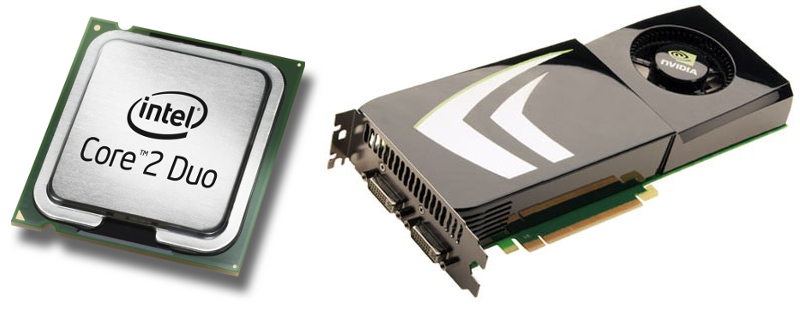
\includegraphics[height=40mm]{img/cpu-gpu.png}
\end{center}

Multi/many-core computing nell'UniPG:

\begin{itemize}
\item INFN: progetto MacGO
\item Fisica, Chimica, \textbf{Informatica}
\end{itemize}
\end{frame}

\begin{frame}{PAES}
Cos'è?
\begin{itemize}
\item Implementazione \textbf{parallela} dell'AES
\item Target: \textbf{CPU} e \textbf{GPU}
\end{itemize}

\vspace{1cm}
Perché?
\begin{itemize}
\item Esplorazione dell'\textbf{hardware}
\item Esplorazione degli \textbf{strumenti}
\item Esplorazione della \textbf{metodologia}
\item Problema reale $\longrightarrow$ ottimo banco di prova
\item Problema reale $\longrightarrow$ risultato riutilizzabile
\end{itemize}
\end{frame}

\begin{frame}{OpenCL}
\begin{center}
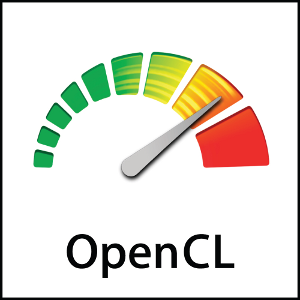
\includegraphics[scale=1]{img/opencl-logo.png}
\end{center}

\begin{itemize}
\item \textbf{Standard} per il multi/many-core computing
\item \textbf{Multi-dispositivo}: CPU, GPU, DSP\ldots{}
\item \textbf{Multi-piattaforma}: Linux, Windows\ldots{}
\end{itemize}
\end{frame}

\begin{frame}{Comprendere OpenCL}
Come può OpenCL astrarre dispositivi così eterogenei?
\begin{enumerate}
\item Modello della \textbf{piattaforma}
\item Modello della \textbf{memoria}
\item Modello di \textbf{esecuzione}
\item Modello di \textbf{programmazione}: parallelismo \textbf{sui dati}
\end{enumerate} 
\end{frame}

\begin{frame}{Modello della piattaforma}
\vspace{5mm}
\begin{center}
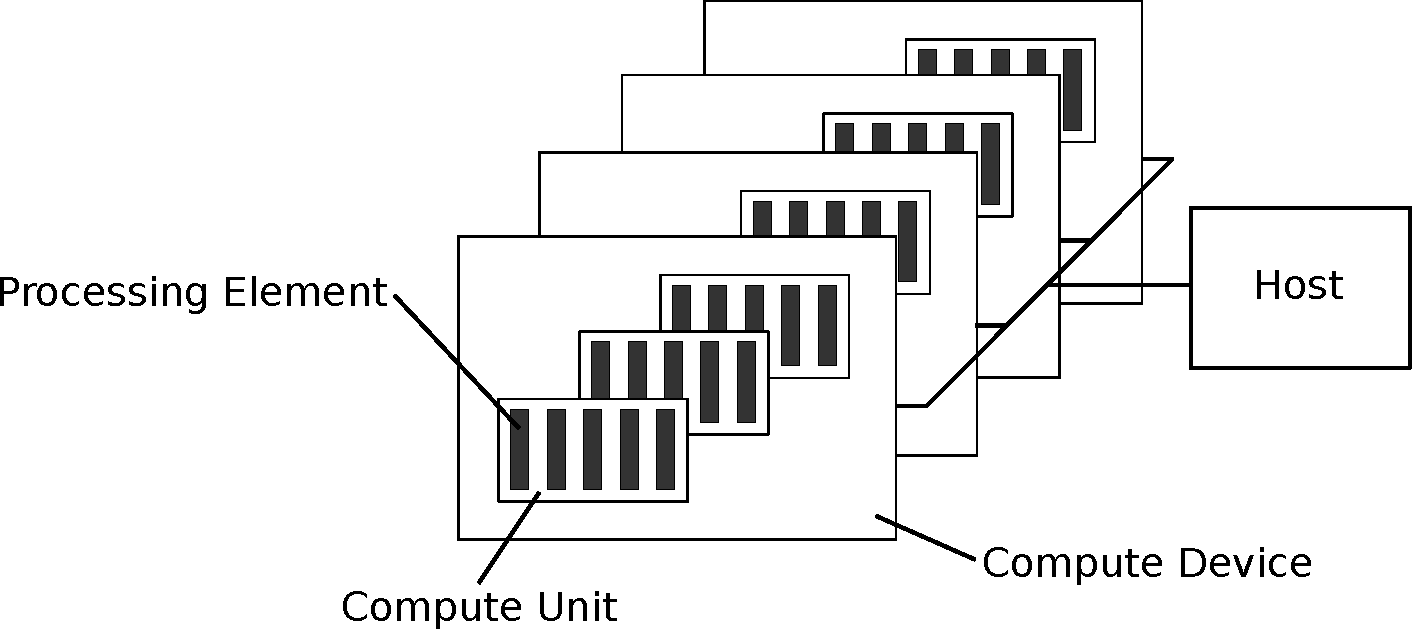
\includegraphics[width=10cm]{img/opencl-platform-model.pdf}
\end{center}
\end{frame}

\begin{frame}{Modello della memoria}
\vspace{3mm}
\begin{center}
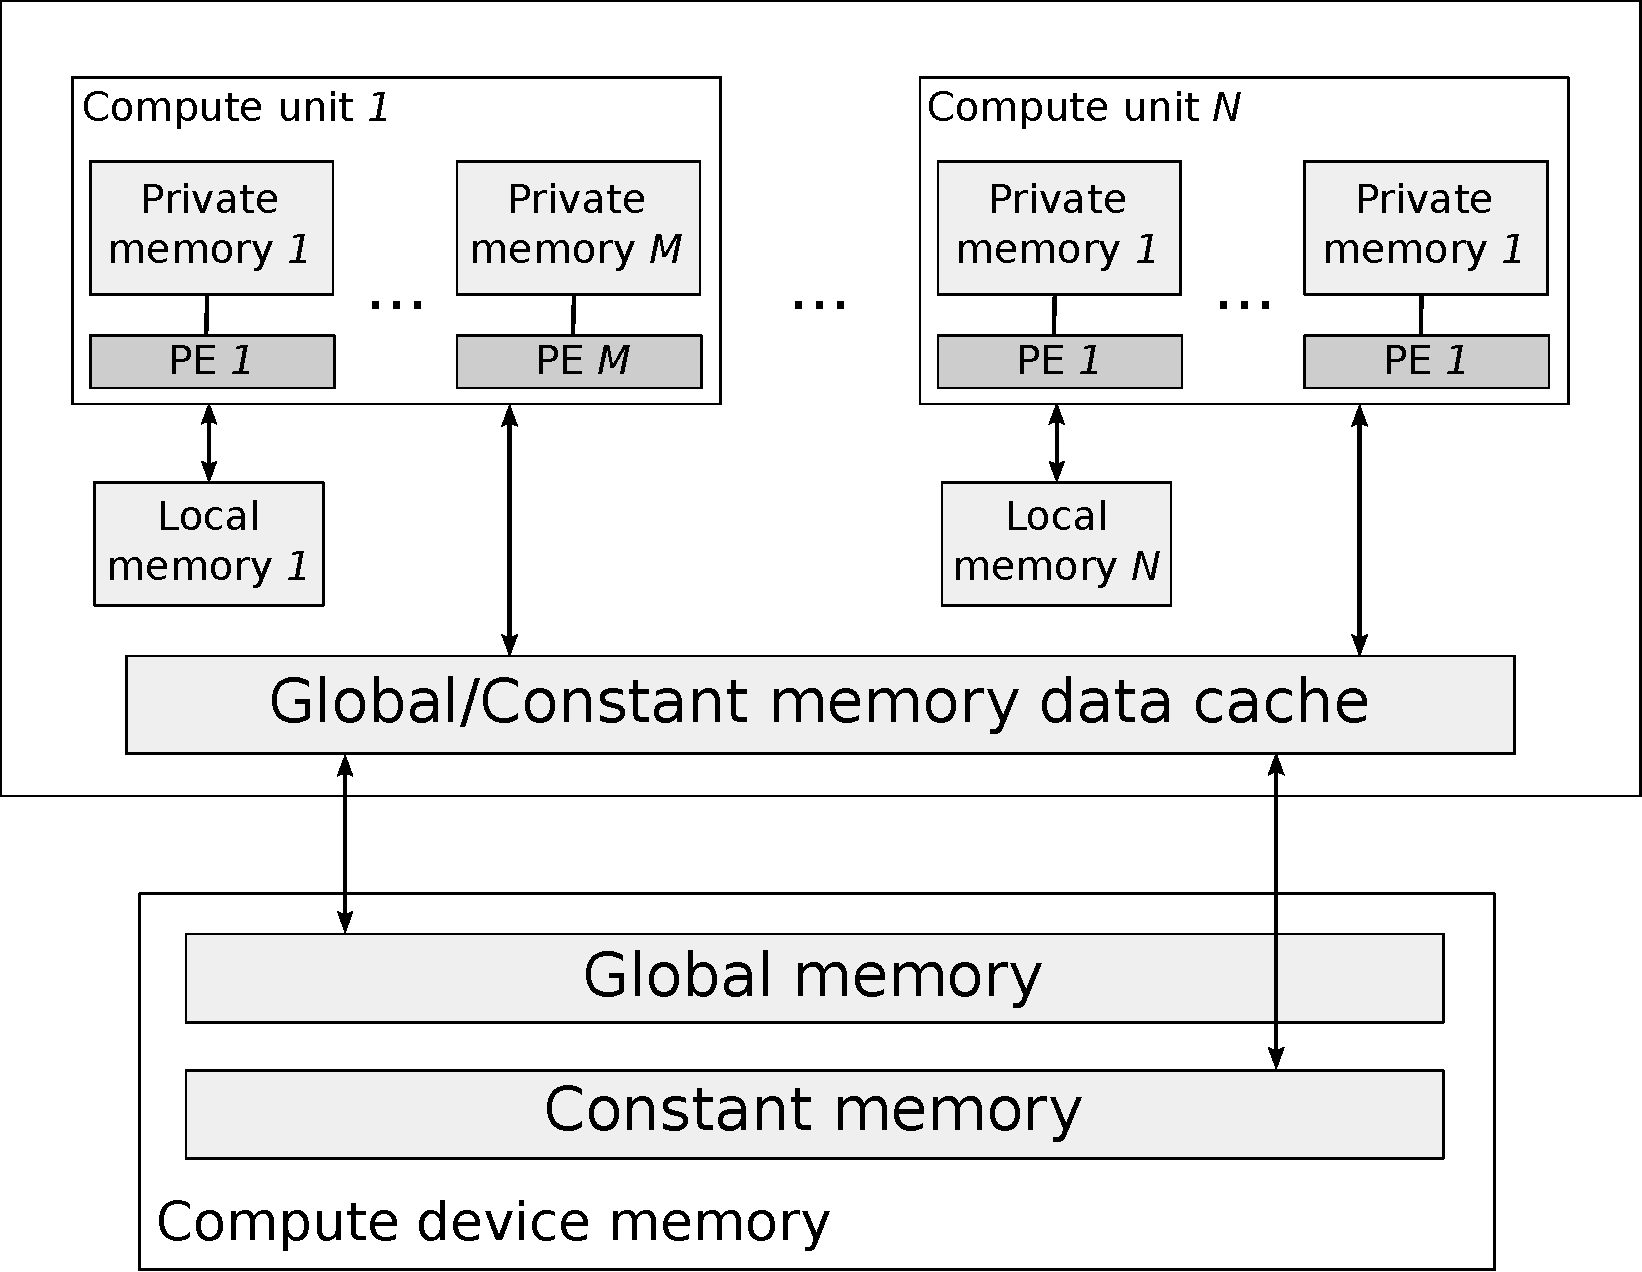
\includegraphics[width=9cm]{img/opencl-memory-model.pdf}
\end{center}
\end{frame}

\begin{frame}{Modello di esecuzione}
I ruoli:
\begin{itemize}
\item L'\textbf{host prepara} l'esecuzione dei \textbf{kernel}
\item Il \textbf{device esegue} i calcoli
\end{itemize}

\vspace{3mm}
I protagonisti:
\begin{itemize}
\item Work-items
\item Work-groups
\end{itemize}

\vspace{3mm}
Due modi per identificare un work-item:
\begin{enumerate}
\item Global ID
\item Work-group ID e Local ID
\end{enumerate}
\end{frame}

\begin{frame}{Estensioni del C per i kernel}
Estensioni del C99:
\begin{itemize}
\item Tipi di dato vettoriali
\item Tipi di dato per le immagini
\item Conformità IEEE-754
\item Modificatori aggiuntivi per la memoria
\end{itemize}

\vspace{4mm}
Limitazioni rispetto al C99:
\begin{itemize}
\item No ricorsione
\item No libreria standard
\item No scrittura mediante puntatori $< 32$ bit
\end{itemize}
\end{frame}

\begin{frame}{AES}
\begin{center}

\includegraphics[width=5cm]{img/nist.pdf}
\end{center}

\vspace{5mm}
Identikit:
\begin{itemize}
\item Standard FIPS-197
\item Algoritmo \textbf{simmetrico}, \textbf{iterato}, a \textbf{blocchi}
\item Blocchi di 128 bit, chiavi di 128, 192 o 256 bit
\end{itemize}
\end{frame}

\begin{frame}[fragile]
\frametitle {Algoritmo di cifratura AES}
\begin{lstlisting}[language=Pascal]
State = input
AddRoundKey(State, RoundKey[0])
for r = 1 to rounds-1
    SubBytes(State)
    ShiftRows(State)
    MixColumns(State)
    AddRoundKey(State, RoundKey[r])
end
SubBytes(State)
ShiftRows(State)
AddRoundKey(State, RoundKey[rounds])
output = State
\end{lstlisting}
\end{frame}

\begin{frame}{Strumenti utilizzati}
Hardware:
\begin{itemize}
\item Intel Core 2 Duo E6300
\item NVIDIA GeForce GTX 275	
\end{itemize}

\vspace{3mm}
Software:
\begin{itemize}
\item Linux (32 e 64 bit)
\item GCC, DDD e Valgrind
\item Framework OpenCL di AMD e NVIDIA
\item Doxygen
\item Python
\end{itemize}

\end{frame}

\begin{frame}{Gestione del parallelismo}
\begin{itemize}
\item Partizionamento naturale sui blocchi
\item Blocchi distribuiti uniformemente ai work-item
\item Ogni work-item cifra $\frac{global~size}{blocchi}$ blocchi
\item L'eventuale resto viene ripartito equamente
\end{itemize}

\vspace{3mm}
\begin{center}
\underline{Evitati limiti \textbf{artificiosi} al numero di work-item e work-group}
\end{center}

\end{frame}

\begin{frame}{Global e local size}
\vspace{4mm}
Nessun vincolo artificioso, quindi:
\begin{itemize}
\item Global e local size \textbf{ottimali per il device}
\item Global e local size \textbf{ottimali per l'input}
\end{itemize}

\vspace{3mm}
Due strategie:
\begin{enumerate}
\item \textbf{Statica}: valori fissi
\item \textbf{Dinamica}: global size = blocchi, local size = $\frac{global~size}{ratio}$
\end{enumerate}

\vspace{8mm}
%\centering\textbf{\textcolor{OliveGreen}{Ottima portabilità su dispositivi eterogenei!}}
\begin{center}
\begin{block}{}
\centering Ottima portabilità su dispositivi eterogenei
\end{block}
\end{center}


\end{frame}

\begin{frame}{Il programma host}
\begin{enumerate}
\item Calcola le \textbf{chiavi di round}
\item \textbf{Prepara l'esecuzione} dei kernel con l'API OpenCL
\item \textbf{Scrive l'input} nella memoria del device
\item Esegue il kernel \textbf{una volta per ciascun round}
\item \textbf{Legge il risultato} dalla memoria del device
\item Rileva i \textbf{tempi di esecuzione}
\end{enumerate}
\end{frame}

\begin{frame}[fragile]
\frametitle{Il kernel di PAES}
\begin{lstlisting}
__kernel __attribute__((vec_type_hint(uchar)))
void kernel_aes(
    __global uchar16 *buffer, 
    const ulong blocks, 
    const uint mode, 
    __constant const uchar16 *round_key, 
    const uint rounds, 
    const uint round)
\end{lstlisting}
\end{frame}

\begin{frame}[fragile]
\frametitle{Funzioni AES: un esempio}
\begin{lstlisting}
__constant const uchar sbox_encrypt[256] = ...
__constant const uchar sbox_decrypt[256] = ...

void sub_bytes(size_t block, 
               __global uchar16 *buffer, 
               __constant const uchar *sbox)
{
    buffer[block] = (uchar16)(
        sbox[buffer[block][0]], 
        ... 
        sbox[buffer[block][15]]);
}
\end{lstlisting}
\end{frame}


\begin{frame}{Testing}
Due tipologie di test:
\begin{enumerate}
\item Correttezza
\item Prestazioni
\end{enumerate}

\vspace{2mm}
\begin{center}
\begin{block}{}
\centering Implementazione seriale single-core di riferimento
\end{block}
\end{center}
Idee di fondo:
\begin{itemize}
\item test frequenti $\rightarrow$ il più automatici possibile
\item test facili da scrivere $\rightarrow$ Python
\end{itemize}
\end{frame}

\begin{frame}{Prestazioni}
\vspace{3mm}
\begin{center}
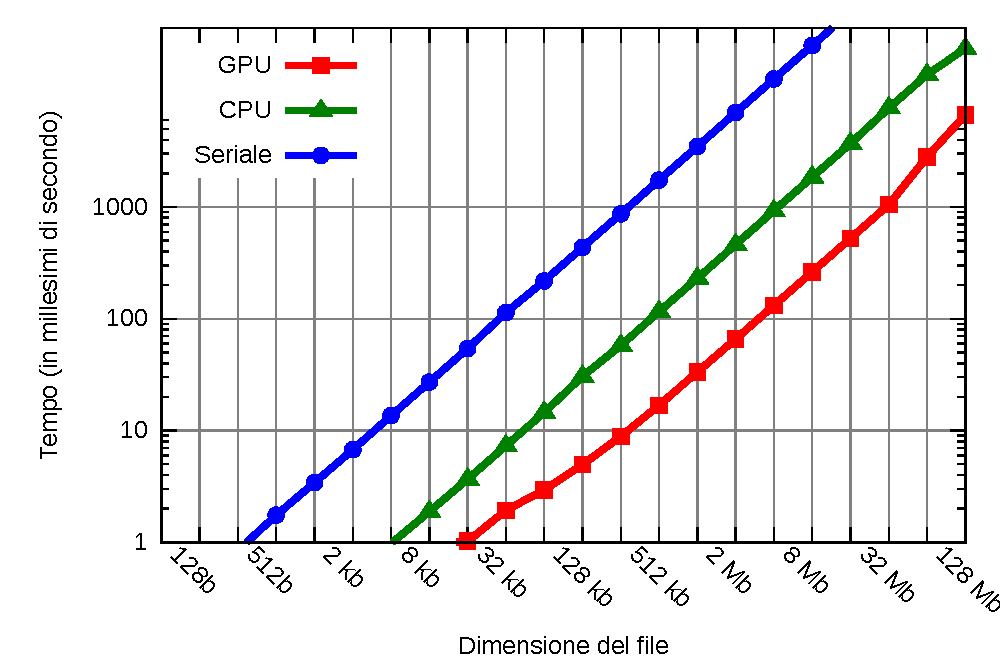
\includegraphics[height=7cm,width=10cm]{img/test-encrypt.pdf}
\end{center}
\end{frame}

\begin{frame}{Comparazione delle prestazioni}
\begin{center}
\begin{tabular}{|r||r|r|r|}
\hline
\textbf{Dimensione (byte)} & \textbf{GPU/CPU} & \textbf{GPU/Seriale} & \textbf{CPU/Seriale} \\
\hline
\hline
\textbf{128} & 0.106 & 0.308 & \textcolor{OliveGreen}{\textbf{\underline{2.893}}} \\
\hline
\textbf{256} & 0.144 & 0.590 & 4.096 \\
\hline
\textbf{512} & 0.213 & \textcolor{OliveGreen}{\textbf{\underline{1.126}}} & 5.287 \\
\hline
\textbf{2048} & 0.316 & 3.773 & 11.941 \\
\hline
\textbf{4096} & 0.575 & 7.414 & 12.889 \\
\hline
\textbf{8192} & \textcolor{OliveGreen}{\textbf{\underline{1.078}}} & 15.039 & 13.945 \\
\hline
\textbf{65536} & 3.776 & 58.791 & 15.014 \\
\hline
\textbf{131072} & 4.936 & 74.110 & 15.125 \\
\hline
\textbf{8388608} & 7.030 & 106.332 & 15.568 \\
\hline
\end{tabular}
\end{center}
\end{frame}

\begin{frame}{Input/output}
\vspace{7mm}
\begin{center}
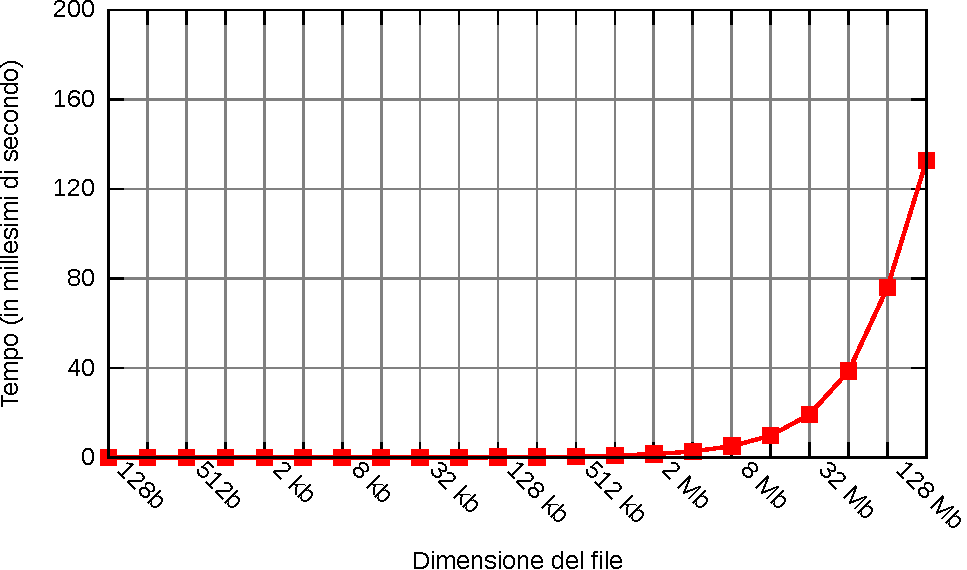
\includegraphics[width=10cm]{img/test-write-gpu.pdf}
\end{center}
\end{frame}

\begin{frame}{Conclusioni}
Metodologia:
\begin{itemize}
\item Dispositivi eterogenei $\rightarrow$ Flessibilità nel parallelismo
\item Framework instabili $\rightarrow$ Sviluppo multi-framework
\item Codice complesso $\rightarrow$ Testing intensivo
\end{itemize}

\vspace{5mm}
Sviluppi futuri:
\begin{itemize}
\item Codice facilmente comprensibile e riutilizzabile
\item OpenSSL $\rightarrow$ Modalità d'uso dei cifrari
\end{itemize}
\end{frame}

\begin{frame}[plain]
\vspace{12mm}
\begin{center}
\textbf{\huge{Grazie per l'attenzione!}}
\end{center}
\end{frame}

\end{document}
